\begin{frame}{Summary}
\begin{figure}
    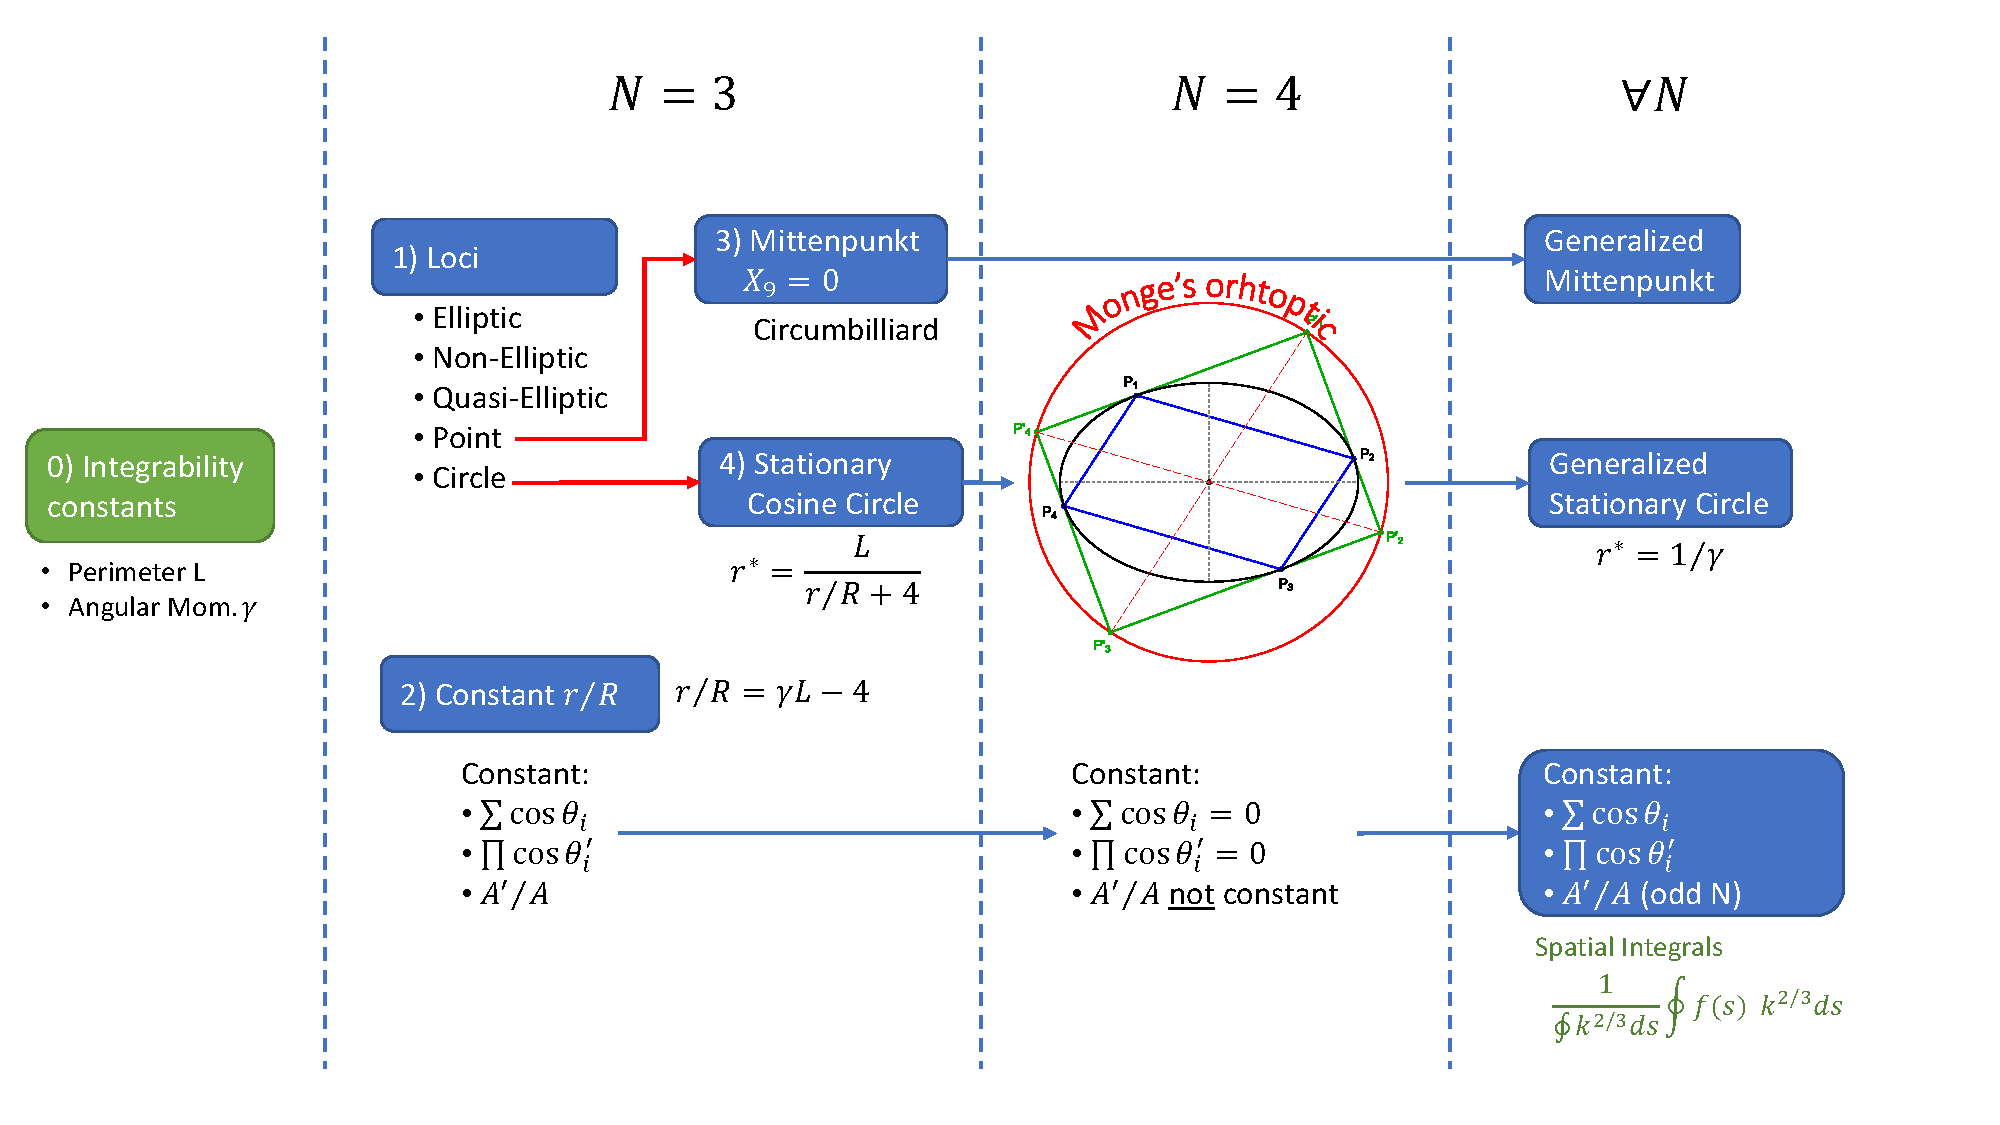
\includegraphics[clip,trim={0 0 0 0},height=.9\textheight]{pics/0002_diagram_slide.pdf}
\end{figure}
\end{frame}

\begin{frame}{Project's \href{https://dan-reznik.github.io/Elliptical-Billiards-Triangular-Orbits/}{[Homepage]}}
\begin{figure}
    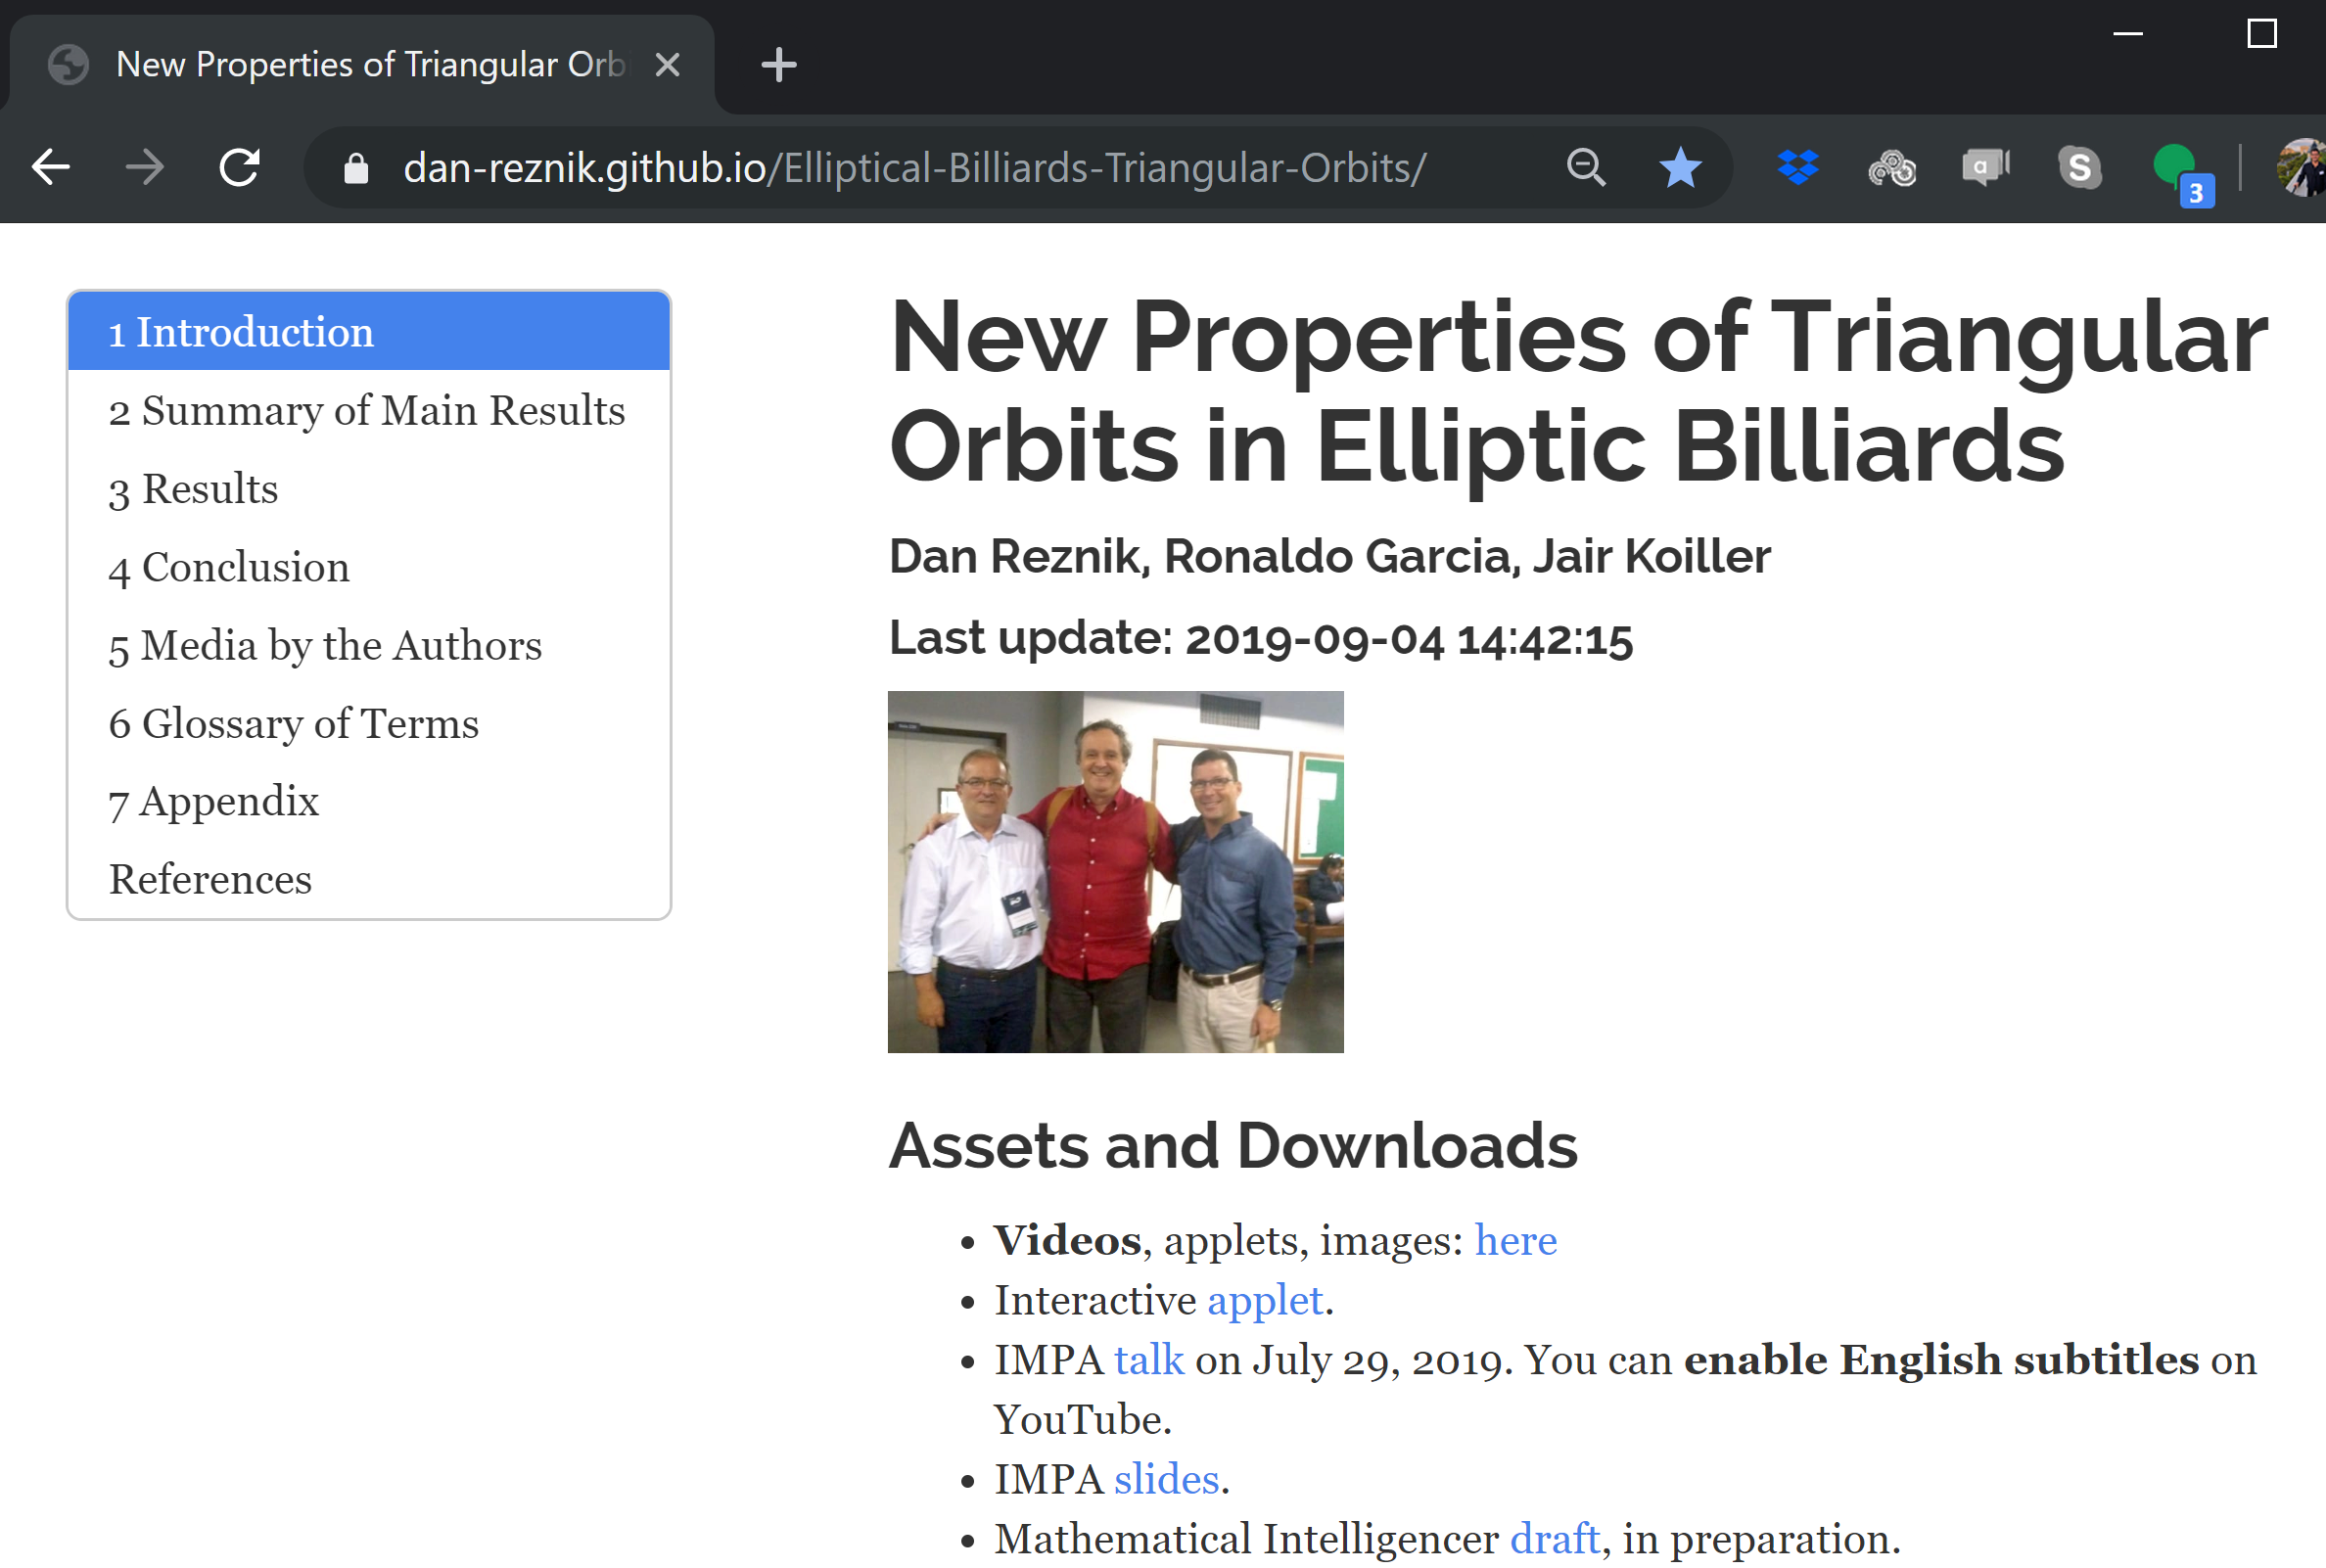
\includegraphics[height=.8\textheight]{pics/0000_website.png}
\end{figure}

\end{frame}

\begin{frame}{Questions}
\begin{itemize}
    \item * $N=3$: why is a locus is elliptic or non?
    \item * Invariants for Ellipsoidal (3d) Billiard?
    \item * Invariants in self-intersecting orbits? (\href{https://youtu.be/cCYxN7ueGV4}{N=4} and \href{https://youtu.be/ECe4DptduJY}{N=5})
    \item * Invariants in non-billiard (Poncelet) orbit families?
    \item * Invariants for orbits on sphere?
\end{itemize}

\vspace*{1cm}

\begin{minipage}{.2\textwidth}
\textbf{Thanks!}
\end{minipage}
\begin{minipage}{.3\textwidth}
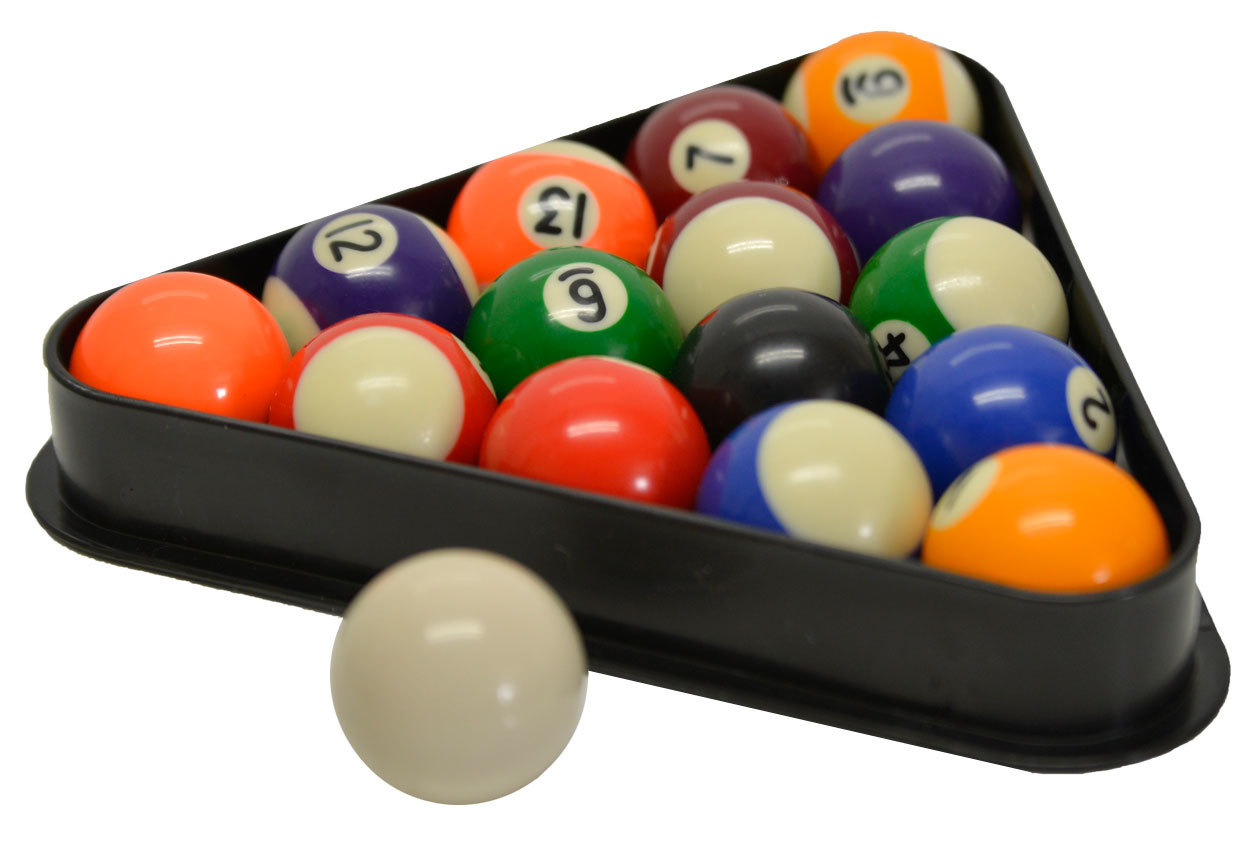
\includegraphics[height=0.25\textheight]{pics/0000_billiard_rack.png} 
\end{minipage}
\begin{minipage}{.4\textwidth}
\href{dreznik@gmail.com}{dreznik[@]gmail[.]com}\\
\href{ragarcia@ufg.br}{ragarcia[@]ufg[.]br}\\
\href{jairkoiller@gmail.com}{jairkoiller[@]gmail[.]com}
\end{minipage}
\end{frame}

